In this section, we discuss the performance of an SPH simulation code
with self-gravity implemented using FDPS. The test problem used is the
simulation of Giant Impact (GI). The giant impact
hypothesis \cite{1975Icar...24..504H, 1976LPI.....7..120C} is one of
the most popular scenarios for the formation of the Moon. The
hypothesis is as follows. About 5 billion years ago, a Mars-sized
object (hereafter, the impactor) collided with the proto-Earth
(hereafter, the target). The collision scattered a large amount of
debris, which first formed the debris disk and eventually the
Moon. Many researchers have performed simulations of GI, using the SPH
method.
\cite{1986Icar...66..515B, 2013Icar..222..200C, 2014NatGe...7..564A}.

For the gravity, we used monopole-only kernel with $\theta=0.5$. We
adopt the standard SPH scheme
\cite{1992ARA&A..30..543M, 2009NewAR..53...78R, 2010ARA&A..48..391S}
for the hydro part. Artificial viscosity is used to handle shock waves
\cite{1997JCoPh.136..298M}, and 
the standard Balsara switch is used to reduce the shear viscosity
\cite{1995JCoPh.121..357B}. Assuming that the target and impactor
consist of granite, we adopt equation of state of
granite \cite{1986Icar...66..515B} for the particles. The initial
conditions, such as the orbital parameters of the two objects, are the
same as those in \cite{1986Icar...66..515B}. In this paper, we report
the weak scaling performance with about 250k particles per node. For
the largest calculation, we used $1.0$ billion particles and $4096$
nodes.

\begin{figure}
  \begin{center}
    \includegraphics[width=8cm]{fig/GI.eps}
  \end{center}
  \caption{Temperature maps of the target and impactor in the run of
  $9.9$ million particles at four different epochs. }
  \label{fig:evolutionGI}
\end{figure}

Figure~\ref{fig:evolutionGI} shows the time evolution of the target
and impactor for a run with 9.9 million particles. We can see that the shock waves
are formed just after the moment of impact in both the target and
impactor (t=2050sec). The shock propagates in the target, while the
impactor is completely disrupted (t=2847sec) and debris is ejected. A
part of the debris falls back to the target, while the rest will
eventually form the disk and the Moon. So far, the resolution used in
the published papers have been much lower. We plan to use this code to
improve the accuracy of the GI simulations.

\begin{figure}
  \begin{center}
    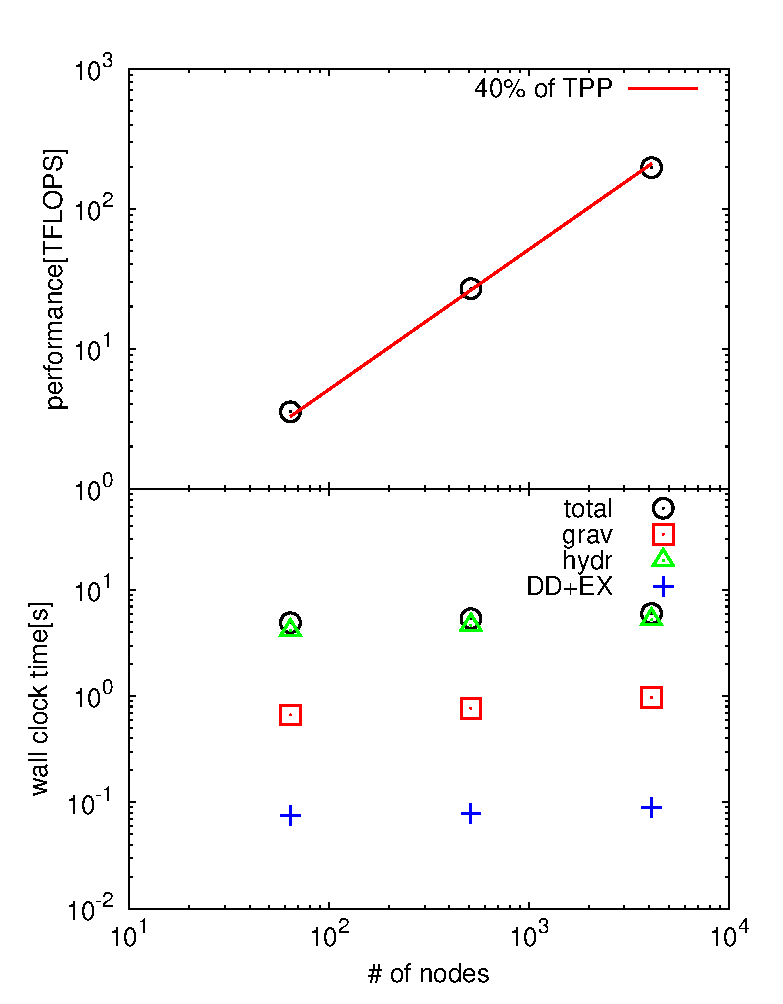
\includegraphics[width=8cm]{fig/bench_gi.eps}
  \end{center}
  \caption{Wallclock time per one timestep plotted as functions of the
    number of nodes. Time spent for hydrodynamics calculation (Hydro),
    and gravity calculation (Grav) are also shown.}
  \label{fig:benchGI}
\end{figure}

Figure~\ref{fig:benchGI} shows the wallclock time per timestep. We
can see the weak-scaling performance is quite good. The hydro part
consumes more time than the gravity part does, mainly because the
particle-particle interaction is more complicated.

The largest number of particles used for GI simulations so far
reported is 100 million \cite{2014LPI....45.2703T}. Unfortunately,
performance numbers are not given. After we replace the interaction
kernels with SIMD-optimized ones for hydrodynamics part, we believe we
can achieve the performance not so much lower than that we achieved
for pure gravity calculation.

% LocalWords:  SPH FDPS impactor proto Balsara rr rrr Grav Wendland SIMD

% LocalWords:  builtin Wallclock timestep wallclock monopole
